\documentclass[11pt]{article}

\usepackage{float}
\usepackage{hyperref}
\usepackage{graphicx}
% formatting
\usepackage{verbatim}
\usepackage{moreverb}
\usepackage{minted}
\usepackage{parskip}
\usepackage{amsmath}
\usepackage[listings]{tcolorbox}
\usepackage{enumerate}
\let\verbatiminput=\verbatimtabinput
\def\verbatimtabsize{4\relax}

\newcommand{\RepoRootPath}{fpga\_labs\_sp20}

\tcbset{
texexp/.style={colframe=black, colback=lightgray!15,
         coltitle=white,
         fonttitle=\small\sffamily\bfseries, fontupper=\small, fontlower=\small},
     example/.style 2 args={texexp,
title={Question \thetcbcounter: #1},label={#2}},
}

\newtcolorbox{texexp}[1]{texexp}
\newtcolorbox[auto counter]{texexptitled}[3][]{%
example={#2}{#3},#1}

\setlength{\topmargin}{-0.5in}
\setlength{\textheight}{9in}
\setlength{\oddsidemargin}{0in}
\setlength{\evensidemargin}{0in}
\setlength{\textwidth}{6.5in}

% Useful macros

\newcommand{\note}[1]{{\bf [ NOTE: #1 ]}}
\newcommand{\fixme}[1]{{\bf [ FIXME: #1 ]}}
\newcommand{\wunits}[2]{\mbox{#1\,#2}}
\newcommand{\um}{\mbox{$\mu$m}}
\newcommand{\xum}[1]{\wunits{#1}{\um}}
\newcommand{\by}[2]{\mbox{#1$\times$#2}}
\newcommand{\byby}[3]{\mbox{#1$\times$#2$\times$#3}}


\newenvironment{tightlist}
{\begin{itemize}
 \setlength{\parsep}{0pt}
 \setlength{\itemsep}{-2pt}}
{\end{itemize}}

\newenvironment{titledtightlist}[1]
{\noindent
 ~~\textbf{#1}
 \begin{itemize}
 \setlength{\parsep}{0pt}
 \setlength{\itemsep}{-2pt}}
{\end{itemize}}

% Change spacing before and after section headers

\makeatletter
\renewcommand{\section}
{\@startsection {section}{1}{0pt}
 {-2ex}
 {1ex}
 {\bfseries\Large}}
\makeatother

\makeatletter
\renewcommand{\subsection}
{\@startsection {subsection}{1}{0pt}
 {-1ex}
 {0.5ex}
 {\bfseries\normalsize}}
\makeatother

% Reduce likelihood of a single line at the top/bottom of page

\clubpenalty=2000
\widowpenalty=2000

% Other commands and parameters

\pagestyle{myheadings}
\setlength{\parindent}{0in}
\setlength{\parskip}{10pt}

% Commands for register format figures.

\newcommand{\instbit}[1]{\mbox{\scriptsize #1}}
\newcommand{\instbitrange}[2]{\instbit{#1} \hfill \instbit{#2}}
\newcommand{\itwos}{I\textsuperscript{2}S}

\begin{document}

\def\PYZsq{\textquotesingle}
\title{\vspace{-0.4in}\Large \bf EECS 151/251A FPGA Lab Spring 2021\\
Lab 4:\\Handshake, FIFO, HDMI Output\vspace{-0.1in}}

\author{Prof. John Wawrzynek \\
TAs: Sean Huang, Tan Nguyen \\ Department of Electrical Engineering and Computer Sciences\\
College of Engineering, University of California, Berkeley}
\date{}
\maketitle

\section{Before You Start This Lab}
You should run \verb|git pull| in \verb|fpga_labs_sp21| to get the latest files for this lab.

Replace the following files with your code from Lab 2.
\begin{itemize}
  \item \verb|lab4/src/debouncer.v|
  \item \verb|lab4/src/synchronizer.v|
  \item \verb|lab4/src/edge_detector.v|
\end{itemize}

In addition, there are some changes to the Memory modules in \verb|lib/EECS151.v|. In particular, an \verb|en| (enable) input pin is added to the \verb|SYNC_RAM| and \verb|SYNC_ROM|, along with some new dual-port memory modules which we introduce later. If you're still working on the previous labs, you should not pull from the lab repository until you're done, or you should ensure that your synchronous memory instantiations set the enable signal to high.

Before you proceed with the contents of this lab, we suggest that you get acquainted with what a \href{http://inst.eecs.berkeley.edu/~eecs151/sp20/files/verilog/ready_valid_interface.pdf}{ready/valid handshake} is. It may be helpful to draw out the timing diagrams for the ready/valid handshake to gain understanding. If you are having trouble, ask a TA. 

In this lab, we will build a FIFO with a Ready/Valid interface (also known as Handshake interface). We will also leverage the Handshake interface to build a simple image streaming pipeline to send a static image stored in the FPGA memory blocks to the HDMI output of the PYNQ board. \textbf{The FIFO module plays a significant role in the success of your final project, so you should test your FIFO implementation rigorously}. For the HDMI task, if you have an HDMI monitor at home, you can try connecting it with your FPGA board to test your design. Nonetheless, the HDMI demo at checkoff is optional, but you will need to ensure that your RTL implementation simulates correctly with the given testbenches and is synthesizable.

\section{Building a Synchronous FIFO}
A FIFO (first in, first out) data buffer is a circuit that allows data elements to be queued through a write interface, and read out sequentially by a read interface.
The FIFO we will build in this section will have both the read and write interfaces clocked by the same clock; this circuit is known as a synchronous FIFO.

\subsection{FIFO Functionality}
A FIFO is implemented with a circular buffer (2D reg) and two pointers: a read pointer and a write pointer.
These pointers address the buffer inside the FIFO, and they indicate where the next read or write operation should be performed.
When the FIFO is reset, these pointers are set to the same value.

When a write to the FIFO is performed, the write pointer increments and the data provided to the FIFO is written to the buffer.
When a read from the FIFO is performed, the read pointer increments, and the data present at the read pointer's location is sent out of the FIFO.

A comparison between the values of the read and write pointers indicate whether the FIFO is full or empty.
You can choose to implement this logic as you please.
The \verb|Electronics| section of the \href{https://en.wikipedia.org/wiki/FIFO_(computing_and_electronics)}{FIFO Wikipedia article} will likely aid you in creating your FIFO.

For your reference, here is a block diagram of the Xilinx FIFO from page 103 of the \href{https://www.xilinx.com/support/documentation/ip_documentation/fifo_generator_ug175.pdf}{Xilinx FIFO IP Manual}.

\begin{center}
    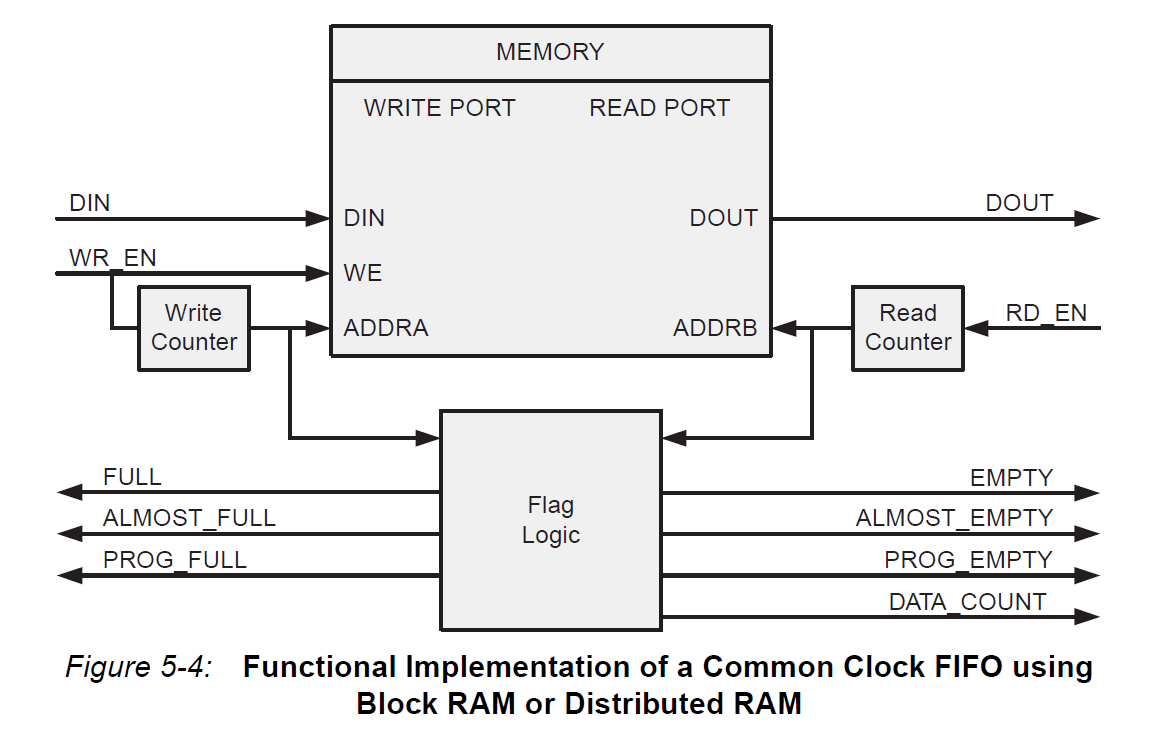
\includegraphics[height=7cm]{figs/sync_fifo_diagram.png}
\end{center}


Our FIFO, however, will have a much simpler interface than this. To make it convenient for you to connect your FIFOs with other Ready/Valid blocks in the future as well as to keep things consistent, our FIFO will also adopt the Ready/Valid Interface for the Read and Write channels. Since it might be read and written at the same time, we have to use a dual-ported memory block which supports two independent memory ports. Take a look at our library file \verb|lib/EECS151.v|, two new dual-port memory modules have been added: \verb|SYNC_RAM_DP| and \verb|ASYNC_RAM_DP|. Either can be used to implement our FIFO buffer. The difference between the two modules is the synchronous memory block requires one-cycle read latency, whereas the read data of the asynchronous memory is available immediately (check Lab 3). You can take a look at their implementations for a better understanding. We use the synthesis attributes to enforce \verb|SYNC_RAM_DP| to map to Block RAMs, while \verb|ASYNC_RAM_DP| gets mapped to LUT RAMs on the FPGA, but the tool makes a final decision based on the availability of the resources. You can check with the Synthesis log file and the final report utilization to make sure you get what you want.


\begin{center}
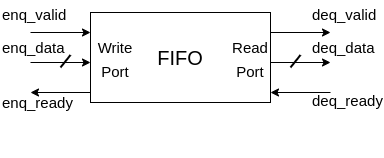
\includegraphics[width=0.4\textwidth]{figs/fifo.png}
\end{center}

\subsection{FIFO Interface}
Look at the FIFO skeleton in \verb|src/fifo.v|.

The FIFO is parameterized by:
\begin{itemize}
    \item \verb|WIDTH|    - The number of bits per entry in the FIFO
    \item \verb|LOGDEPTH| - The log2 of number of entries in the FIFO. For simplicity, our FIFO has a depth of power-of-two values.
\end{itemize}

The common FIFO signals are:
\begin{itemize}
    \item \verb|clk| - Clock used for both read and write interfaces of the FIFO.
    \item \verb|rst| - Reset (synchronous with \verb|clk|); should force the FIFO to become empty.
\end{itemize}

The FIFO write (or "enqueue") interface consists of:
\begin{itemize}
    \item \verb|input enq_valid| - If this signal is HIGH, the \verb|enq_data| is valid to be written to the FIFO (necessary, but not sufficient condition).
    \item \verb|input [WIDTH-1:0] enq_data| - the data to be written to the FIFO.
    \item \verb|output enq_ready| - If this signal is LOW, the FIFO is currently full. Nothing can be written to the FIFO. In other word, the FIFO is not ready to be enqueued/written to yet. \textbf{Use this signal to indicate whether the FIFO is full or not}.
\end{itemize}

The FIFO read (or "dequeue") interface consists of:
\begin{itemize}
    \item \verb|input deq_ready| - If this signal is HIGH, the \verb|deq_data| is ready to be read from the FIFO (necessary, but not sufficient condition).
    \item \verb|output [WIDTH-1:0] deq_data| - the data to be read from the FIFO.
    \item \verb|output deq_valid| - If this signal is LOW, the FIFO is currently empty. Nothing can be read from the FIFO. In other word, the \verb|deq_data| is an invalid data to be dequeued/read from the FIFO. \textbf{Use this signal to indicate whether the FIFO is empty or not}.
\end{itemize}

These signals work as similar to what you read from the \href{http://inst.eecs.berkeley.edu/~eecs151/sp20/files/verilog/ready_valid_interface.pdf}{ready/valid handshake} document. One way to imagine how it works is, for example, you can assume that the FIFO connects to a Source block (producing the data to the FIFO) on the Write interface, and a Sink block (consuming the data from the FIFO) on the Read interface. Therefore,

\begin{itemize}
    \item If \verb|enq_valid| and \verb|enq_ready| are both HIGH at a clock rising edge, the current data \verb|enq_data| from the Source block should be written/transferred to the FIFO at \textbf{the same} clock rising edge (enqueue "fired"). There is a handshake between the producer (writer) and the FIFO write interface. The write address increments at \textbf{the same} clock rising edge. Otherwise, nothing should be written to the FIFO.
    \item If \verb|deq_valid| and \verb|deq_ready| are both HIGH at a clock rising edge, the data \verb|deq_data| should be latched/transferred to the Sink block at \textbf{the same} clock rising edge (dequeue "fired"). There is a handshake between the FIFO read interface and the consumer (reader). The read address increments at \textbf{the same} clock rising edge. Otherwise, nothing should be read from the FIFO.
\end{itemize}

When you are confused whether a read or write transfer should happen, one tip is to always only look at the signal values right at a particular \textbf{rising edge}. Is Ready HIGH? Is Valid HIGH? If yes to both, the data on the FIFO data pin (\verb|enq_data| or \verb|deq_data|) is transferred at that rising edge. You don't really need to pay attention to how they change during that \textbf{clock cycle} prior to the rising edge. Read the linked document again to make sure you thoroughly understand how Ready/Valid interface works. If you're still in doubt, ask a TA for more clarification.

\textbf{Your task is to implement the FIFO logic in} \verb|lab4/src/fifo.v|. You will use the \verb|ASYNC_RAM_DP| memory block as the buffer storage for your FIFO module.
You should try to implement a high-performant FIFO, i.e., there should be no cycle delay between any writes or reads in a row if the FIFO is not full or not empty, respectively.

\subsection{FIFO Testing}
We have provided a testbench in \verb|lab4/sim/fifo_tb.v|.

The testbench performs the following test sequence:
\begin{enumerate}
    \item Checks initial conditions after reset (FIFO not full and is empty)
    \item Generates random data which will be used for testing
    \item Pushes the data into the FIFO, and checks at every step that the FIFO is no longer empty
    \item When the last piece of data has been pushed into the FIFO, it checks that the FIFO is not empty and is full
    \item Verifies that cycling the clock and trying to overflow the FIFO doesn't cause any corruption of data or corruption of the full and empty flags
    \item Reads the data from the FIFO, and checks at every step that the FIFO is no longer full
    \item When the last piece of data has been read from the FIFO, it checks that the FIFO is not full and is empty
    \item Verifies that cycling the clock and trying to underflow the FIFO doesn't cause any corruption of data or corruption of the full and empty flags
    \item Checks that the data read from the FIFO matches the data that was originally written to the FIFO
    \item Prints out test debug info
\end{enumerate}

Next are some harder tests:

\begin{itemize}
    \item Several times in a row, write to, then read from the FIFO with no clock cycle delays.
      This will test the FIFO in a way that it's likely to be used when buffering user I/O.

    \item Writing and Reading from the FIFO on the same cycle. We use fork-join to create parallel processes of writing and reading from the FIFO.
\end{itemize}

You should make sure that you pass all the tests before moving on.

\subsection{FIFO with IOs}

Your FIFO passes all the behavioral simulation tests. Well done! Next, we will make sure your FIFO is synthesizable by Vivado and it is actually working on an FPGA. We will do this by using the PYNQ IOs as both the source and the sink for the FIFO. In particular,

\begin{itemize}
    \item We use the buttons to enqueue data to the FIFO. Each \verb|BUTTONS[3:0]| corresponds to a number from \{1, 2, 4, 8\}.
    \item We use the LEDS to show the dequeued data.
    \item When SWITCHES[1] is ON, the PYNQ does not have valid data to enqueue to the FIFO. If \verb|BUTTONS[3]| is pressed, the FIFO is reset to empty.
    \item When SWITCHES[1] is OFF, and any of the buttons is pressed, the PYNQ produces valid data to enqueue to the FIFO
    \item When SWITCHES[0] is OFF, it takes a second to dequeue an entry from the FIFO and display on the LEDS.
    \item When SWITCHES[0] is ON, the PYNQ is not ready to dequeue the data from the FIFO.
\end{itemize}

We have provided the code \verb|lab4/src/z1top_fifo_io.v| for you. Create a project with this file as top-level module and generate a bitstream to test it on the PYNQ. Make sure you add all necessary files (include the \verb|button_parser|, your FIFO code, and the constraint file). Alternatively, you can also run the scripts that we provide to interact with Vivado in command-line mode.

\begin{minted}{bash}
# You should run these commands under ./lab4 directory
# The commands here are optional. If you want to stick with Vivado GUI,
# you don't need to run them.

# This command creates 'z1top_fifo_io' project
make build-project proj=z1top_fifo_io

# This command runs Vivado simulation with the 'fifo_tb' testbench
# To see the waveform, you will need to open the Vivado project
make sim proj=z1top_fifo_io tb=fifo_tb

# This command runs Synthesis, Implementation, and Generate Bitstream
make write-bitstream proj=z1top_fifo_io

# This command loads the bitstream to a connected FPGA
# If you are programming the FPGA using the HW Server, before running this command,
# make sure that you change the port number in lab4/scripts/program_fpga.tcl to your
# assigned port number (check Lab 1)
make program-fpga bs=bitstream_files/z1top_fifo_io.bit

\end{minted}

At some point, if you'd like to see the GUI, you can open the project file \verb|*.xpr| with Vivado.

You can test your FIFO by pressing different buttons, and keep track of the sequence of LEDS display to see if they match. Turn off \verb|SWITCHES[1]|, try writing invalid data to the FIFO. Turn on \verb|SWITCHES[1]| and \verb|SWITCHES[0]| to try filling the FIFO until full, and then slide it off to drain the FIFO. In the next lab and project, your FIFO will receive user input from a keyboard and echo it back via a serial interface; anything can go wrong if your FIFO does not work reliably. It might be helpful to verify the functionality of your FIFO with this simple design beforehand, and you will have an easier time when working on the final project.

\subsection{Questions}\label{sec:Q1}
\begin{enumerate}
\item \textit{Draw} a block diagram of your FIFO design (please do not copy paste the diagram from the Schematic view of Vivado!). If you use FSM to design the control logic for your FIFO, please also include the state transition diagram. Please write a few sentences on how your FIFO module works and how you handle some edge cases.
\item If you used the \verb|SYNC_RAM_DP| module to implement the buffer of the FIFO, would your current design still work correctly and why? If not, how would you redesign it? You don't have to provide a full working implementation; a few sentences to justify your ideas is fine (include figures if needed).
\end{enumerate}

\section{HDMI Output Display}

In this section, we will ask you to build a display controller to interface with the HDMI output port on the PYNQ. Concretely, we stream a static image stored in the ROM of the FPGA to the display controller to the display monitor via HDMI interface. For this lab exercise, your display controller is expected to support a target resolution of 800$\times$600 with a frame-rate of 60Hz. This configuration should work with the monitors in the lab for check-off. As we move forward, you will find out that it is actually not difficult to build a parameterized display controller that can virtually support any resolution and frame-rate if we know all the necessary parameters and do the math right.

It might sound daunting at first, but we'd like to convince you that it is accomplishable thanks to the third-party \verb|rgb2dvi| IP from Digilent. The PYNQ HDMI ports (Input and Output) directly connect to the FPGA fabric via IO bank, and the \verb|rgb2dvi| IP is responsible for generating appropriate TMDS signals to the FPGA IOs that eventually interfaces with a HDMI sink monitor (or DVI). You can read more from the PYNQ documentation \href{https://reference.digilentinc.com/reference/programmable-logic/pynq-z1/reference-manual#hdmi}{HDMI}. You can also learn about the Digilent IP and how it is implemented from their \href{https://github.com/Digilent/vivado-library}{Github repository}. However, it is not required to know all the detail of the IP to actually use it. We just need to provide correct video-related signals to make the IP happy and do the work of streaming video data to the display device for us. Taking advantage of existing IPs saves countless hours of development effort. The signals that we need to pay attention to are:

\begin{itemize}
  \item \verb|vid_pData|: the three-color channel 24-bit video data. Each color channel has 8 bits. The color order is R, B, and G (from MSB to LSB).
  \item \verb|vid_pHSync|: the video Horizontal Syncing signal.
  \item \verb|vid_pVSync|: the video Vertical Syncing signal.
  \item \verb|vid_pVDE|: the video Enable signal (or video active).
\end{itemize}

Let's take a look at the following video timing figure (from \href{https://www.xilinx.com/support/documentation/ip_documentation/v_tc/v6_2/pg016_v_tc.pdf}{Xilinx Video Timing Controller document}) to understand where those signals come from.

\begin{center}
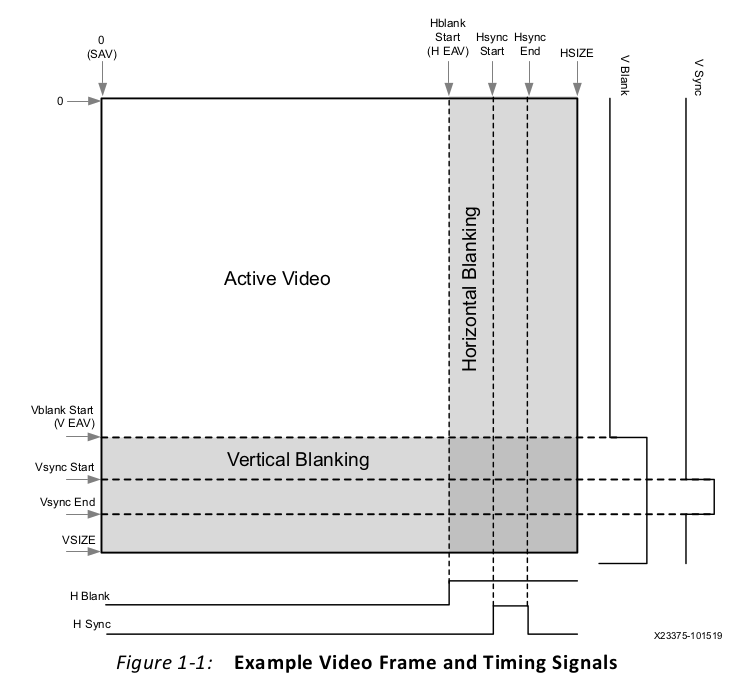
\includegraphics[width=0.6\textwidth]{figs/video_timings.png}
\end{center}

The figure defines the video timing parameters of a video frame. To understand it, you need to be aware that the way of how typical video display works is the pixels are rasterized/scanned from left-to-right, and top-to-bottom. When the display scans a pixel within a region defined in the figure, we assert the corresponding video signals accordingly. Note that the display resolution is actually the \verb|Active Video| region as seen in the figure. Therefore, there are some blanking periods in both horizontal and vertical direction that the display is not supposed to output any pixels. When you look at the spec of a particular display resolution, you will typically find the following parameters:

\begin{itemize}
  \item Horizotal Active Video: from 0 to the Width of the resolution, or HBlank Start.
  \item Horizontal Front Porch: from HBlank Start to HSync Start.
  \item Horizontal Sync Width: from HSync Start to HSync End.
  \item Horizontal Back Porch: from HSync End to HSIZE
  \item Vertical Active Video: from 0 to the Height of the resolution, or VBlank Start.
  \item Veritical Front Porch: from VBlank Start to VSync Start.
  \item Vertical Sync Width: from VSync Start to VSync End.
  \item Vertical Back Porch: from VSync End to VSIZE
\end{itemize}

Open the file \verb|lab4/src/display_controller.v|. You will see the parameters of different display configurations in the Verilog module parameter declarations. These parameters are the multiples of the \textbf{pixel clock cycle}. The pixel clock is calculated based on the target frame-rate (or refresh-rate, e.g., a frame-rate of 60Hz means 60 frames per second) and the \textbf{entire video frame}. Note that a video frame includes both the active region and the blanking region. The pixel clock is the time it takes to emit a single pixel. Thus, with a total of \verb|frame_rate| $\times$ \verb|HSIZE| $\times$ \verb|VSIZE| pixels displayed in a second, a pixel clock can be calculated as 1 / (\verb|frame_rate| $\times$ \verb|HSIZE| $\times$ \verb|VSIZE|) second. As an example, for our target display resolution of 800$\times$600 @60Hz, the frame size is 1056x628 (including blanking regions), and the pixel clock is 25 ns or 40 MHz.

From these known parameters, we can calculate the syncing and blanking timings. As an example, HSync Start can be computed as Horizontal Active Video + Horizontal Front Porch, and HSync End is HSync Start + Horizontal Sync Width.

To interface with the \verb|rgb2dvi| IP properly, we need to assert and deassert the \verb|HSync|, \verb|VSync|, and \verb|VDE| signals according to the spec. The \verb|HSync| should only be HIGH within the Horizontal Sync Width period (HSync Start $\rightarrow$ HSync End), the \verb|VSync| should only be HIGH within the Vertical Sync Width period (VSync Start $\rightarrow$ VSync End), and the \verb|VDE| should only be HIGH within the Active Video period (both horizontal and vertical). We don't care about VBlank or HBlank since the IP does not use these signals.

\subsection{Display controller with FIFO}

The following diagram depicts the system that we would like to run on the FPGA.

\begin{center}
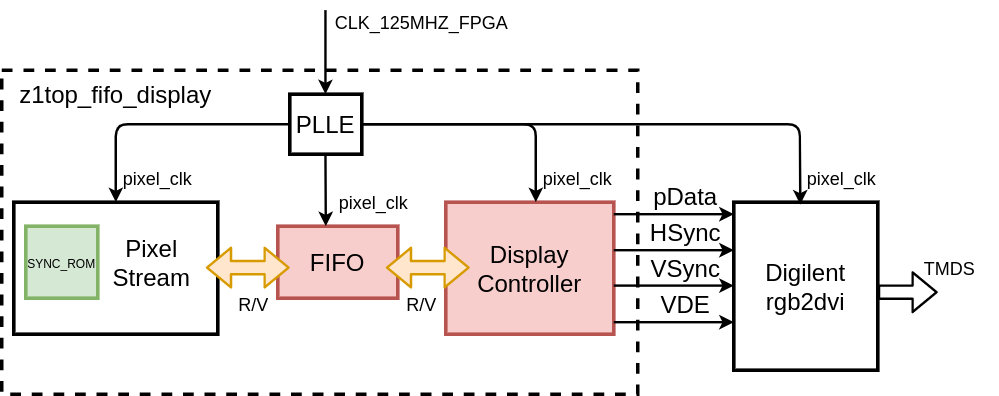
\includegraphics[width=0.6\textwidth]{figs/z1top_fifo_display.png}
\end{center}

The system consists of a pixel streaming block that sends pixel data of an image stored in a ROM every clock cycle to a FIFO. A display controller reads the pixel data from the FIFO and communicates with the Digilent IP to display image on a connected display device. You are responsible for the \verb|FIFO| (from Part 2) and the \verb|display_controller| modules; the remaining blocks are provided to you and you should not need to modify them. Note that your \verb|FIFO| and \verb|display_controller| are now clocked with the pixel clock (40 MHz) instead of the system clock (125 MHz). The pixel clock is generated from the \verb|PLLE| module acting as a clock synthesizer to output a 40 MHz clock from an input 125 MHz clock. We won't go into detail of it for now, but you should keep in mind that there are many ways to generate clock signals on the FPGA.

In summary, the \verb|pixel_stream| is a producer which sends a stream of pixels stored in the ROM to your FIFO. The \verb|display_controller| is a consumer which reads data from your FIFO if it is not empty, and generates video signals for the \verb|rgb2dvi| IP core. Since we are dealing with an IP, we won't be creating Vivado project by just adding Verilog files. Vivado also provides an \texttt{IP Integrator} feature allowing designers to connect their modules at the block level. You can run the script that we provide you to build the block design and genearte the bitstream automatically. Nonetheless, if you'd like to understand the entire process and what it takes, check out the Appendix \ref{section:ipi} for how to use Vivado IP Integrator for this lab exercise. It should create the project with all the modules connected properly.

Your \textbf{first task} is to implement a display controller in \verb|lab4/src/display_controller.v| that conforms to the video signal timings described above. You do not need to read from the FIFO for now, instead, you should write a constant video output (e.g., 24'h00FF00) to the \verb|rgb2dvi| module. \textbf{This should only require a few lines of code}.

Once you have implemented the display controller, run the following script to generate the project and simulate your design with the testbench \verb|lab4/sim/display_controller_tb.v| to make sure that you assert the video timing signals correctly (\verb|HSync|, \verb|VSync|, \verb|VDE|).

\begin{minted}{bash}
# You should run these commands under ./lab4 directory

# This command creates 'z1top_fifo_display' project
make build-project proj=z1top_fifo_display

# This command runs Vivado simulation with the 'display_controller_tb' testbench
# To see the waveform, you will need to open the Vivado project
make sim proj=z1top_fifo_display tb=display_controller_tb

# This command runs Synthesis, Implementation, and Generate Bitstream
make write-bitstream proj=z1top_fifo_display
\end{minted}

It is recommended that you run the scripts under the Linux development environment, such as the lab machines or the VM. If you are using Windows, in case the commands do not work, you can work with GUI as usual. You can follow the Appendix \ref{section:ipi} to create the project with Vivado IPI. Alternatively, you can source the TCL scripts to build the project. Open Vivado GUI, under the TCL Console at the bottom, type

\begin{minted}{bash}
# This only applies to Windows' users
# This command will build the project, add all the necessary source files, and
# perform IP integration with the rgb2dvi Digilent IP
vivado -mode batch -source scripts/build_project.tcl -tclargs z1top_fifo_display
\end{minted}

Please feel free to let the TA know if you have any technical issues with the tools or scripts.

You might want to open up the Vivado project to inspect what actually happens (or look at the script under \verb|lab4/scripts/z1top_fifo_display.tcl|). Click \emph{Open Block Design} under \emph{IP Integrator} to see the high-level overview of the design as shown below.

\begin{center}
\fbox{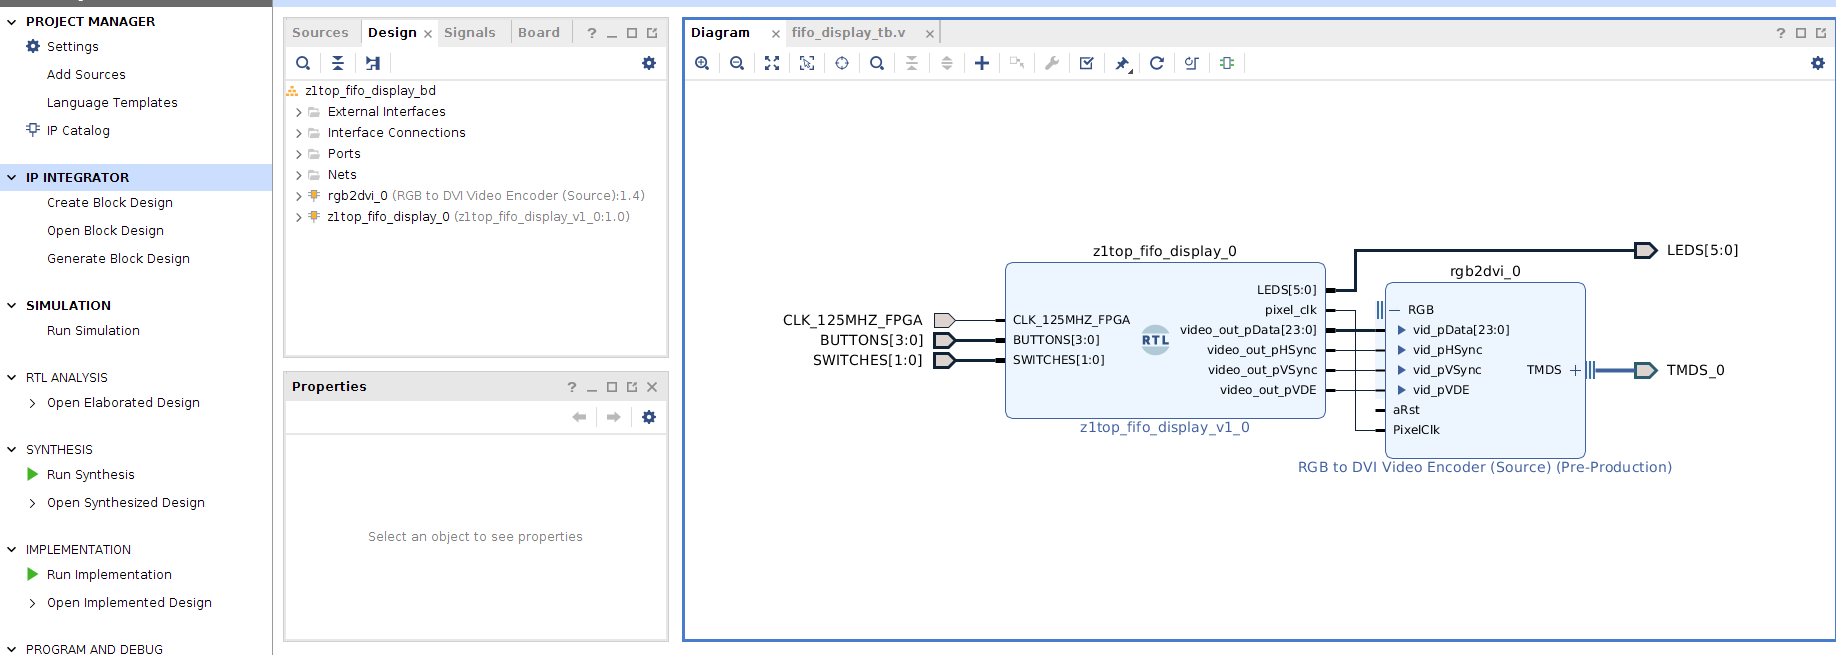
\includegraphics[width=0.8\textwidth]{figs/block_design.png}}
\end{center}

Note that when you use Vivado GUI, before generating bitstream, click on \textbf{Refresh Changed Modules} to make sure Vivado get the latest update of your source files whenever you modify them.

If you successfully generate a bitstream, you can download it to an FPGA using the following command. You can skip this step if you don't wish to test your design on the board with an HDMI monitor.

\begin{minted}{bash}
# If you are programming the FPGA using the HW Server, before running this command,
# make sure that you change the port number in lab4/scripts/program_fpga.tcl to your
# assigned port number (check Lab 1)
make program-fpga bs=bitstream_files/z1top_fifo_display.bit
\end{minted}

If you implement the video timing signals correctly, when you program the FPGA and hook it up with a monitor, it will display a blank green screen on the monitor (or a different color depending on which constant value). That means your display controller works properly. Good work! You can move on to the next part.

Next, your \textbf{second task} is to extend the display controller code to support the Handshake interface that reads pixel data from the FIFO. You are only required to modify the display controller, and you should reuse the FIFO module that you have implemented in Part 2. You need to test your design with the testbench \verb|lab4/sim/fifo_display_tb.v|.

\begin{minted}{bash}
# This command runs Vivado simulation with the 'fifo_display_tb' testbench
# To see the waveform, you will need to open the Vivado project
make sim proj=z1top_fifo_display tb=fifo_display_tb
\end{minted}

As long as you pass the simulation, you can skip the programming FPGA step if you do not wish to test your design on the board. However, please make sure that you can generate bitstream from your design.

You don't need to worry about the implementations or the timings of other blocks in the system. That's the nice thing of Ready/Valid or Handshake interface (often referred to as "Decoupled Interface" in other hardware construction language such as Chisel). All you need is to make sure your display controller can properly enqueue the incoming pixel data for video display, and stop dequeuing during blanking periods. This test sytem also stresses your FIFO implementation in different ways as well, since there will be moments when the FIFO keeps writing and reading data continuously (during video active period), and there is some moment when the FIFO is buffering the data (during the video blanking periods).

If you do everything right, once you program the FPGA, turn on the \verb|SWITCHES[1:0]|, and press \verb|BUTTONS[2]|, you should see a static 800$\times$600 image on your monitor. Next, turn off the \verb|SWITCHES[1:0]| and use the \verb|BUTTONS| to switch between different color channels. As you do the analysis in one of the lab report questions, you will find that the PYNQ does not have enough resource to stream a full RGB 800$\times$600 frame to the display. That would require storing the frame on off-chip DRAM and handling off-chip memory accesses, but let's leave that issue to another day. Your FIFO is good to go and you should be ready for checkoff!

\subsection{Questions}\label{sec:Q2}
\begin{enumerate}
\item In the final task, we nearly exhaust the entire BlockRAM resource to store a 800$\times$600 grayscale image. If we would like to store and stream an RGB image of the same resolution, how many 36Kb-BRAM blocks do we need?
\item If we throw away the FIFO and connect \verb|pixel_stream| module directly to the display controller with the handshake interface, would the system still work (the image can be streamed correctly to the display device)? And why do you think so?
\item If the \verb|pixel_stream| module dropped the handshake support (i.e, it continuously emits a pixel every clock cycle), how would you size the FIFO to ensure steady image streaming with the 800$\times$600 resolution?
\item Besides streaming an image to the display, we also would to like draw some overlay objects (things that you might have seen from some Augmented Reality applications). How would you go about modifying your display controller to overlay an object (e.g., a rectangle) on the image to the display device? Briefly justify your ideas.
\end{enumerate}

%\newpage
\section{Lab Deliverables}
\subsection{Lab Checkoff (due: 11.00AM, Feb 24th, 2021)}
To checkoff for this lab, have these things ready to show the TA:
\begin{enumerate}
  \item Demonstrate that your FIFO implementation passes all the simulation tests in the provided FIFO testbench.
  \item Demonstrate that your FIFO works properly with buttons, switches, and LEDs (\verb|z1top_fifo_io.v|).
  \item Demonstrate that your FIFO can receive the pixel stream and send the pixel stream to the display steadily ( \verb|z1top_fifo_display.v|). You can either show this by displaying correct image output on an HDMI monitor connecting to your PYNQ board, or passing the testbenches \verb|lab4/sim/display_controller_tb.v| and \verb|lab4/sim/fifo_display_tb.v|. Your implementation must also be synthesizable (i.e., it can generate bitstream).
\end{enumerate}

\subsection{Lab Report (due: 11.59PM, Feb 24th, 2021)}\label{sec:labreport}
\begin{enumerate}
  \item Your answers to the questions in sections \ref{sec:Q1} and \ref{sec:Q2}.
\end{enumerate}

\appendix
\section{Using Vivado IP Integrator}
\label{section:ipi}
%Stay tuned.

This appendix will walk you through how to use Vivado IP Integrator (IPI) to create
a design. Vivado IPI enables us to compose a hardware design at a block level, and
facilitates the connection of the hardware blocks by hand or TCL commands. 

First, create a project and add your source files as usual. For this lab, make sure that you add the following files

\verb|lab4/src/button_parser.v|, \verb|lab4/src/synchronizer.v|,

\verb|lab4/src/edge_detector.v|, \verb|lab4/src/debouncer.v|,

\verb|lab4/src/fifo.v|, \verb|lab4/src/fifo_display.v|,

\verb|lab4/src/pixel_stream.v|, \verb|lab4/src/display_controller.v|,

\verb|lab4/src/clk_wiz.v|, \verb|lab4/src/colors.vh|,

\verb|lab4/src/z1top_fifo_display.v|, \verb|lab4/src/ucb_wheeler_hall_bin.mif|,

\verb|lib/EECS151.v|

as \textit{Source files}

and add the constraint file \verb|lab4/constr/z1top.xdc| as \textit{Constraint files}.

Next, click \emph{Create Block Design} under \emph{IP Integrator} in the \emph{Flow Navigator} column.
It will create an empty block design with a default name "design\_1.bd"

\begin{center}
\fbox{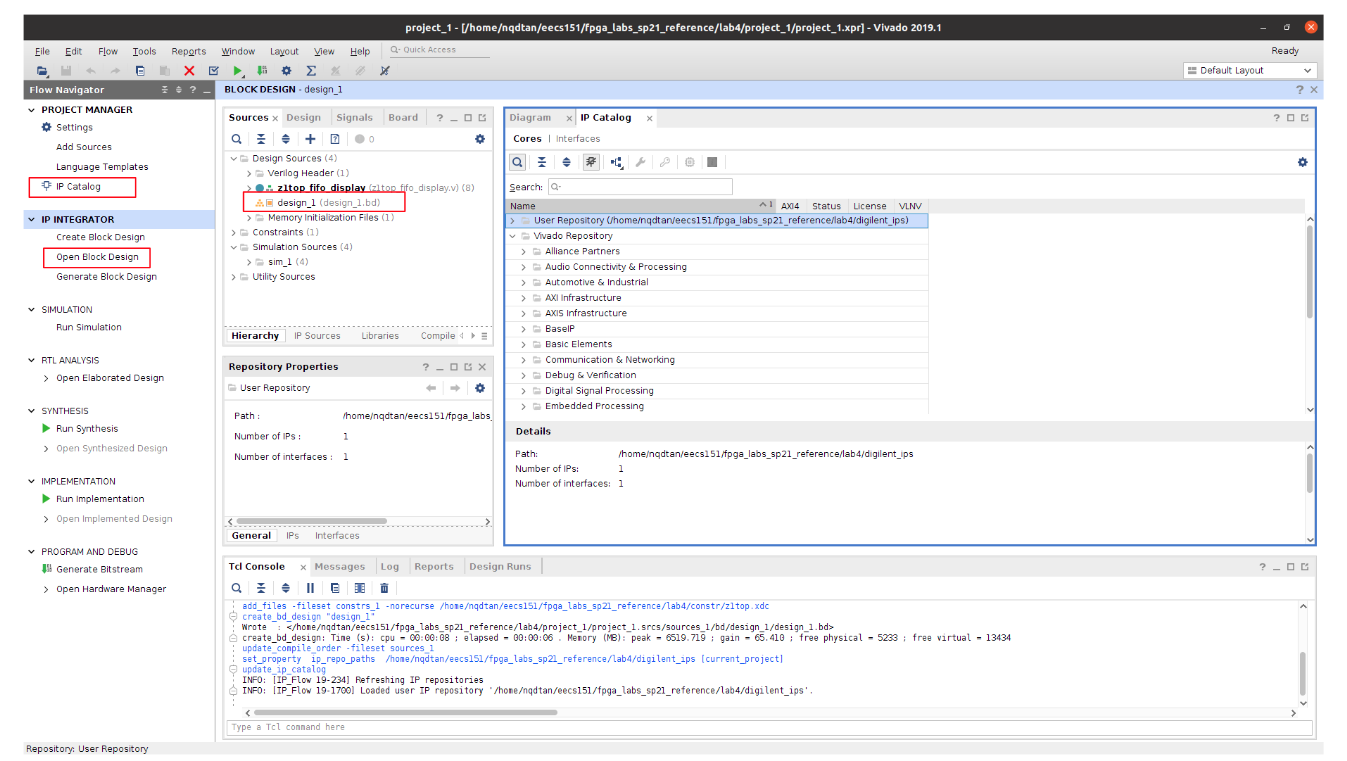
\includegraphics[width=0.6\textwidth]{figs/bd0.png}}
\end{center}

Next, click \emph{IP Catalog} under \emph{Project Manager} in the \emph{Flow Navigator} column.
In the \texttt{IP Catalog} pane, right click then select \emph{Add Repository}. Specify the path
to the Digilent IPs (\verb|lab4/digilent_ips|), then hit \emph{Select}.

Next, click \emph{Open Block Design} under \emph{IP Integrator} to open the block design canvas.
Right click on the \verb|z1top_fifo_display| module in the \textit{Sources} pane, then
select \emph{Add Module to Block Design}. Your RTL core will appear as a "black box" in the
block design canvas.

\begin{center}
\fbox{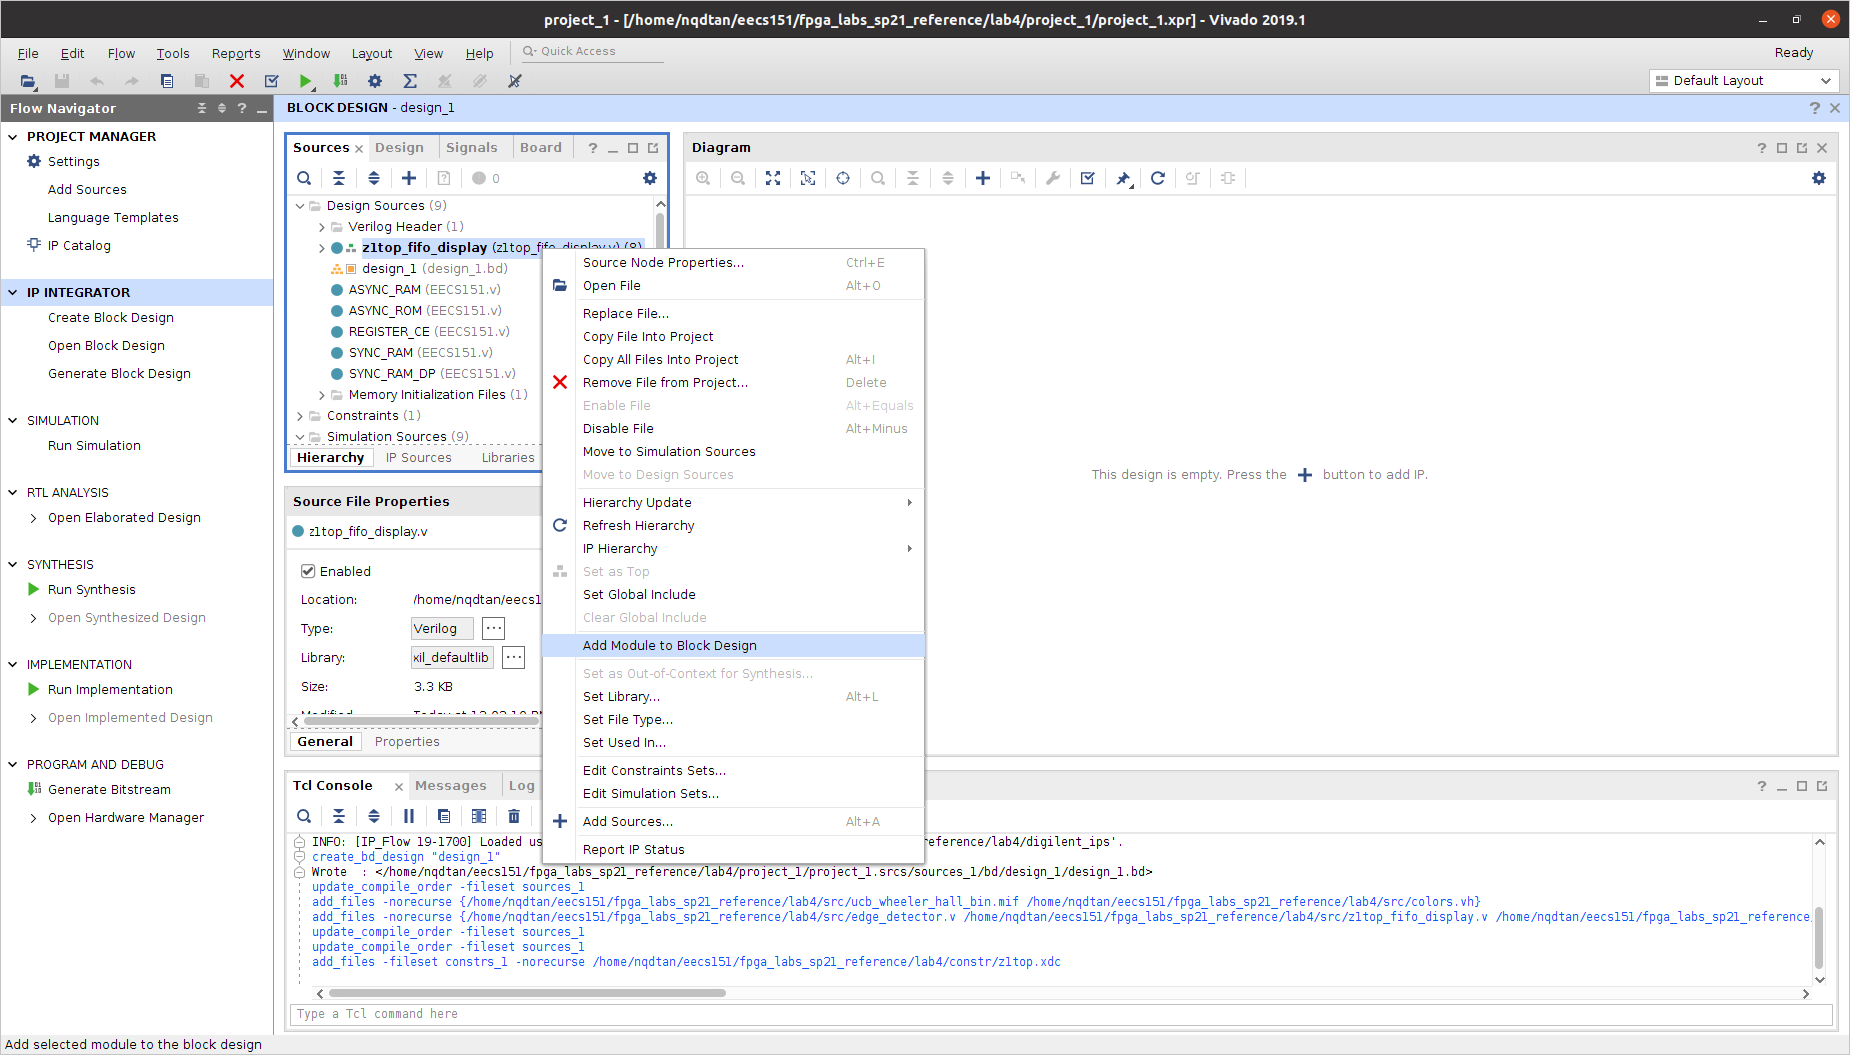
\includegraphics[width=0.7\textwidth]{figs/bd1.png}}
\end{center}

We proceed to add the Digilent video IP. Right click anywhere on the canvas, select \emph{Add IP}.
A dialog will appear. It provides a list of IPs available in Vivado. Since we already added
the Digilent IP, Vivado should be able to find it. Type "digilent" in the search box,
click the IP name to add it to the block design canvas as shown below.

\begin{center}
\fbox{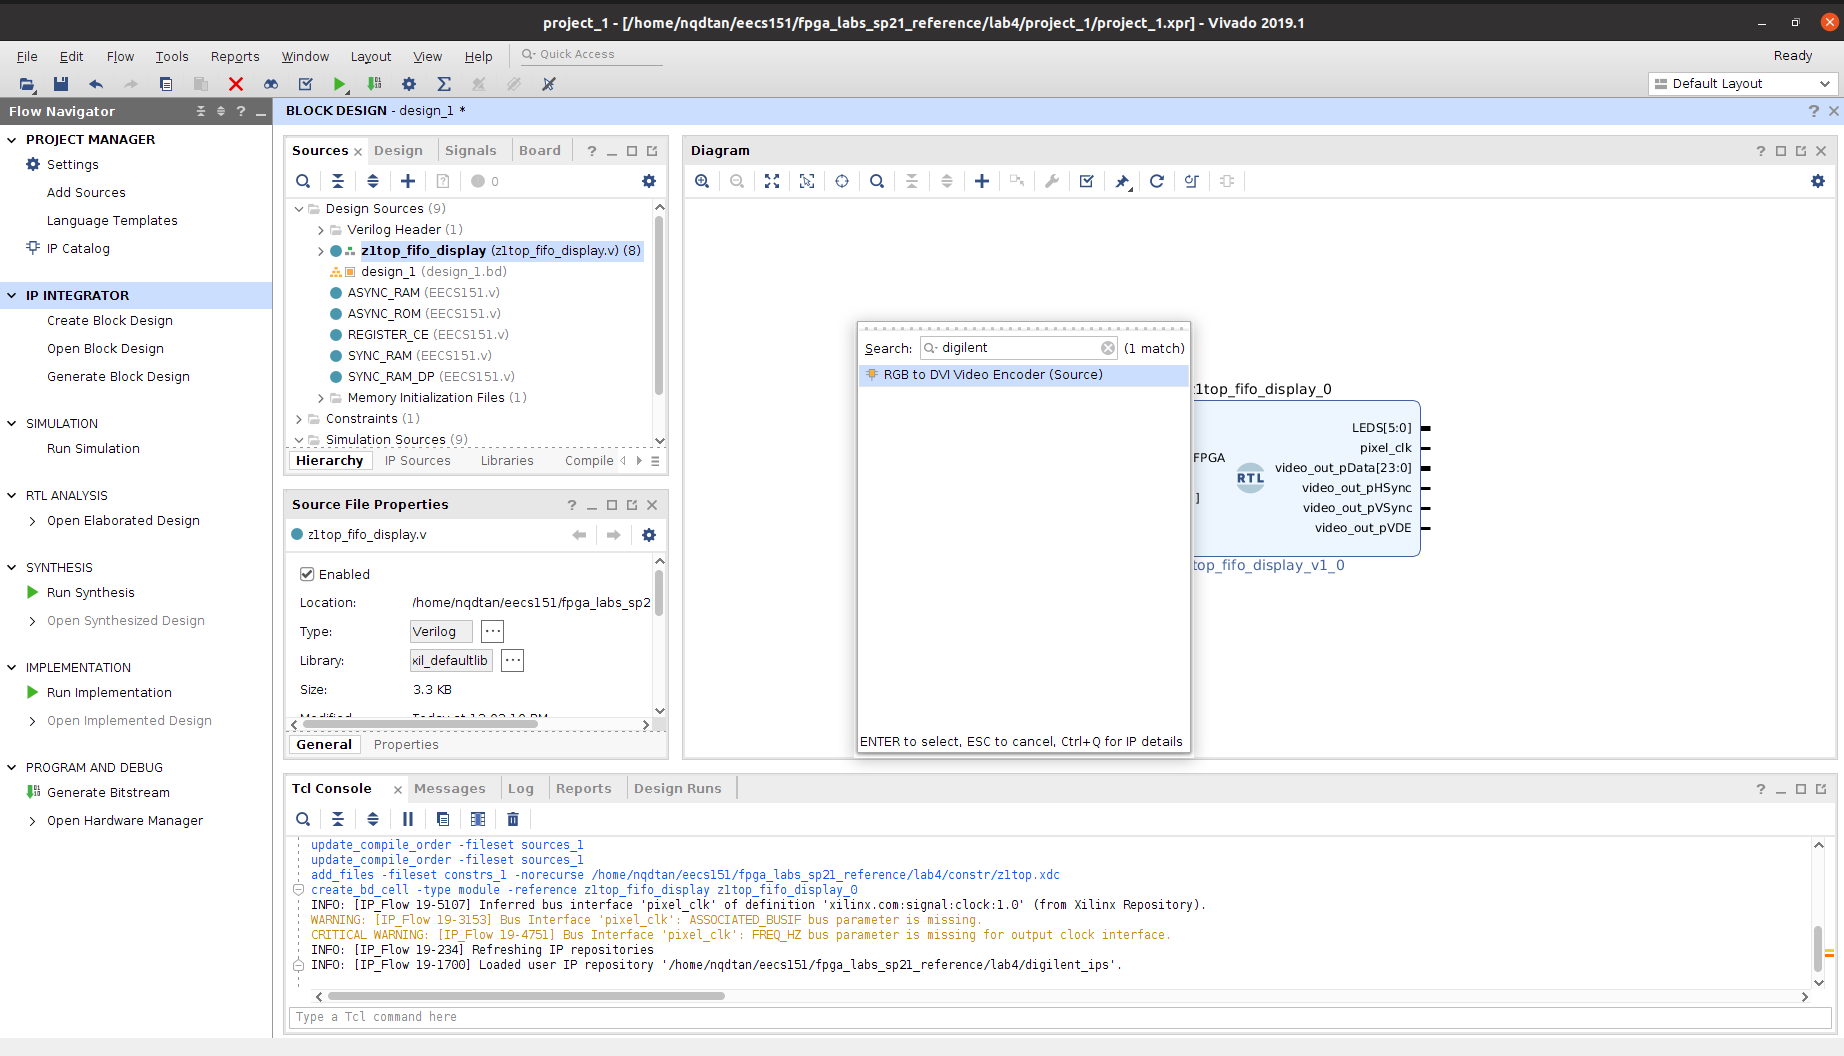
\includegraphics[width=0.7\textwidth]{figs/bd2.png}}
\end{center}

Vivado block design presents to you the block-level view of your modules. Here, you only see the input and output pins of each of the blocks. Connect the blocks as follows.

\begin{enumerate}
\item \texttt{pixel\_clk} goes to \texttt{PixelClk}
\item \texttt{video\_out\_pData} goes to \texttt{vid\_pData} (you need to expand the RGB interface to see the full list of IO ports)
\item \texttt{video\_out\_pHSync} goes to \texttt{vid\_pHSync}
\item \texttt{video\_out\_pVSync} goes to \texttt{vid\_pVSync}
\item \texttt{video\_out\_pVDE} goes to \texttt{vid\_pVDE}
\item You can ignore the pin \texttt{aRst} of the \texttt{rgb2dvi} IP
\end{enumerate}

\begin{center}
\fbox{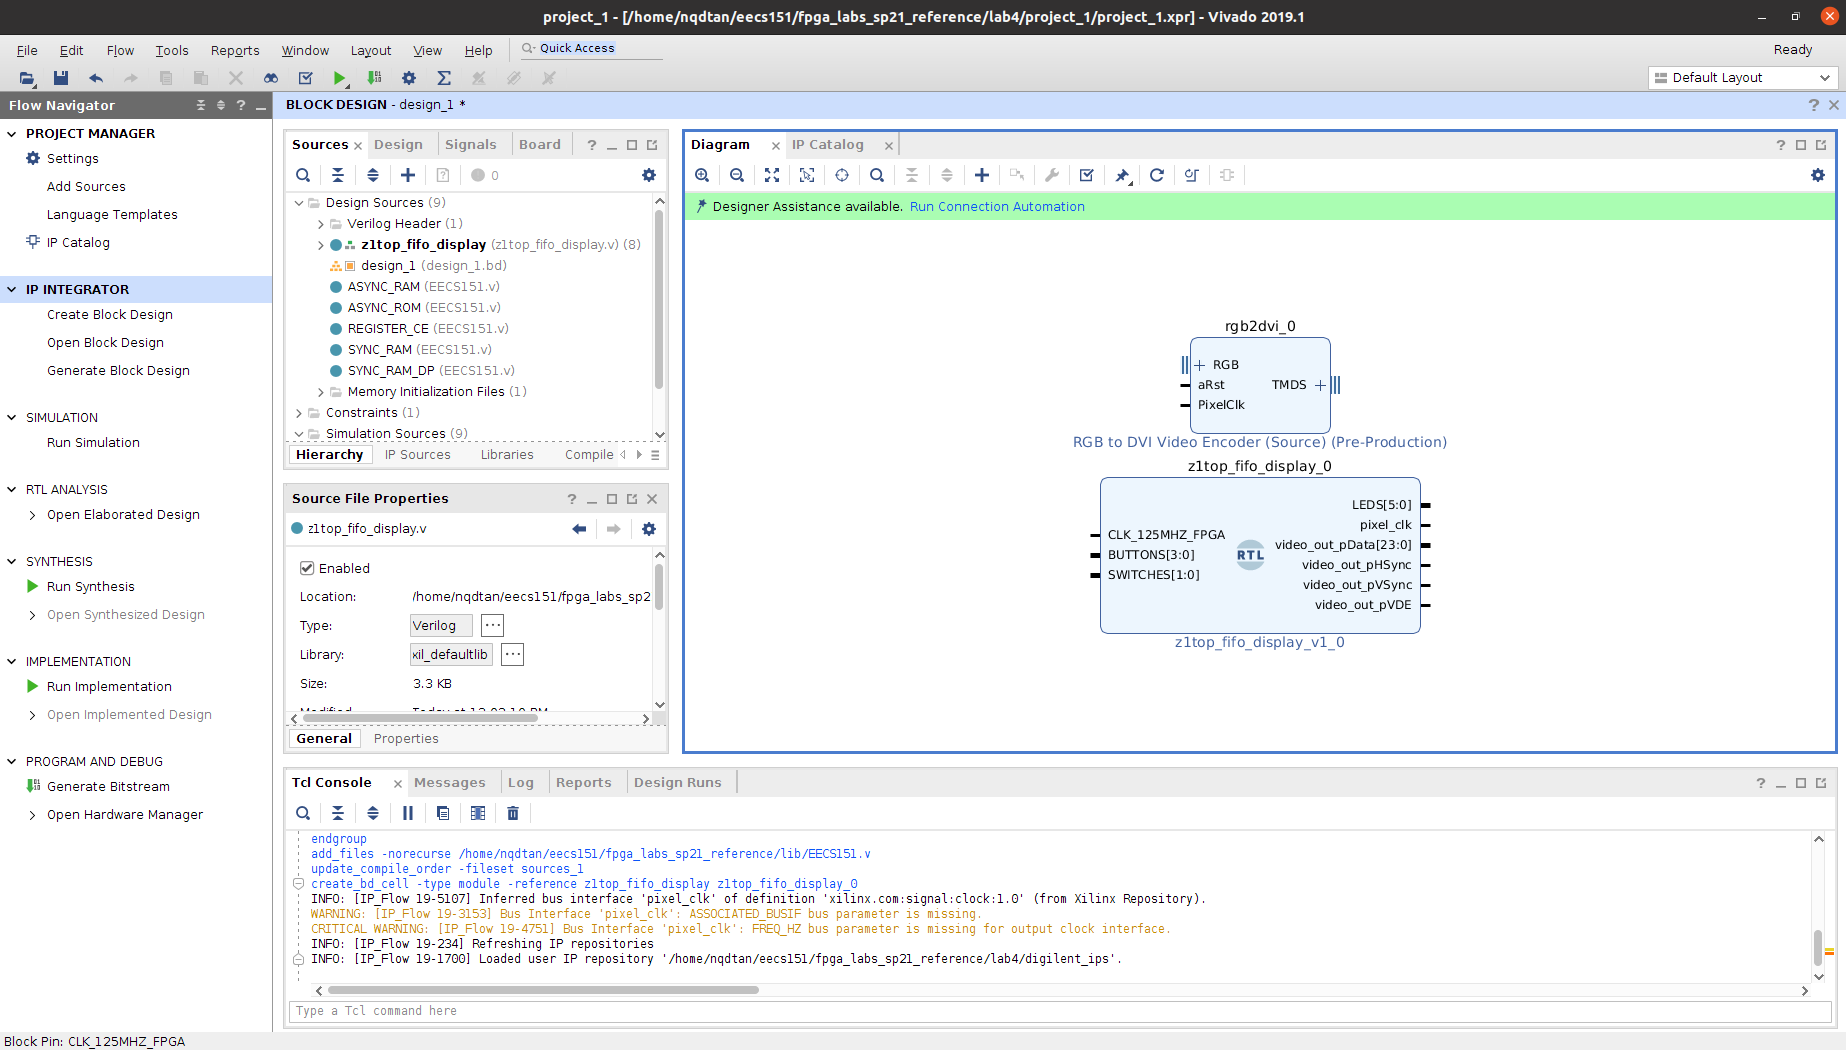
\includegraphics[width=0.7\textwidth]{figs/bd3.png}}
\end{center}

Next, click on the ports \texttt{CLK\_125MHZ\_FPGA}, \texttt{BUTTONS[3:0]}, \texttt{SWITCHES[1:0]}, \texttt{LEDS[1:0]}, and \texttt{TMDS}. Right click and select
\emph{Make External}. Vivado will create the block design's input and output pins that connect to those ports.

\begin{center}
\fbox{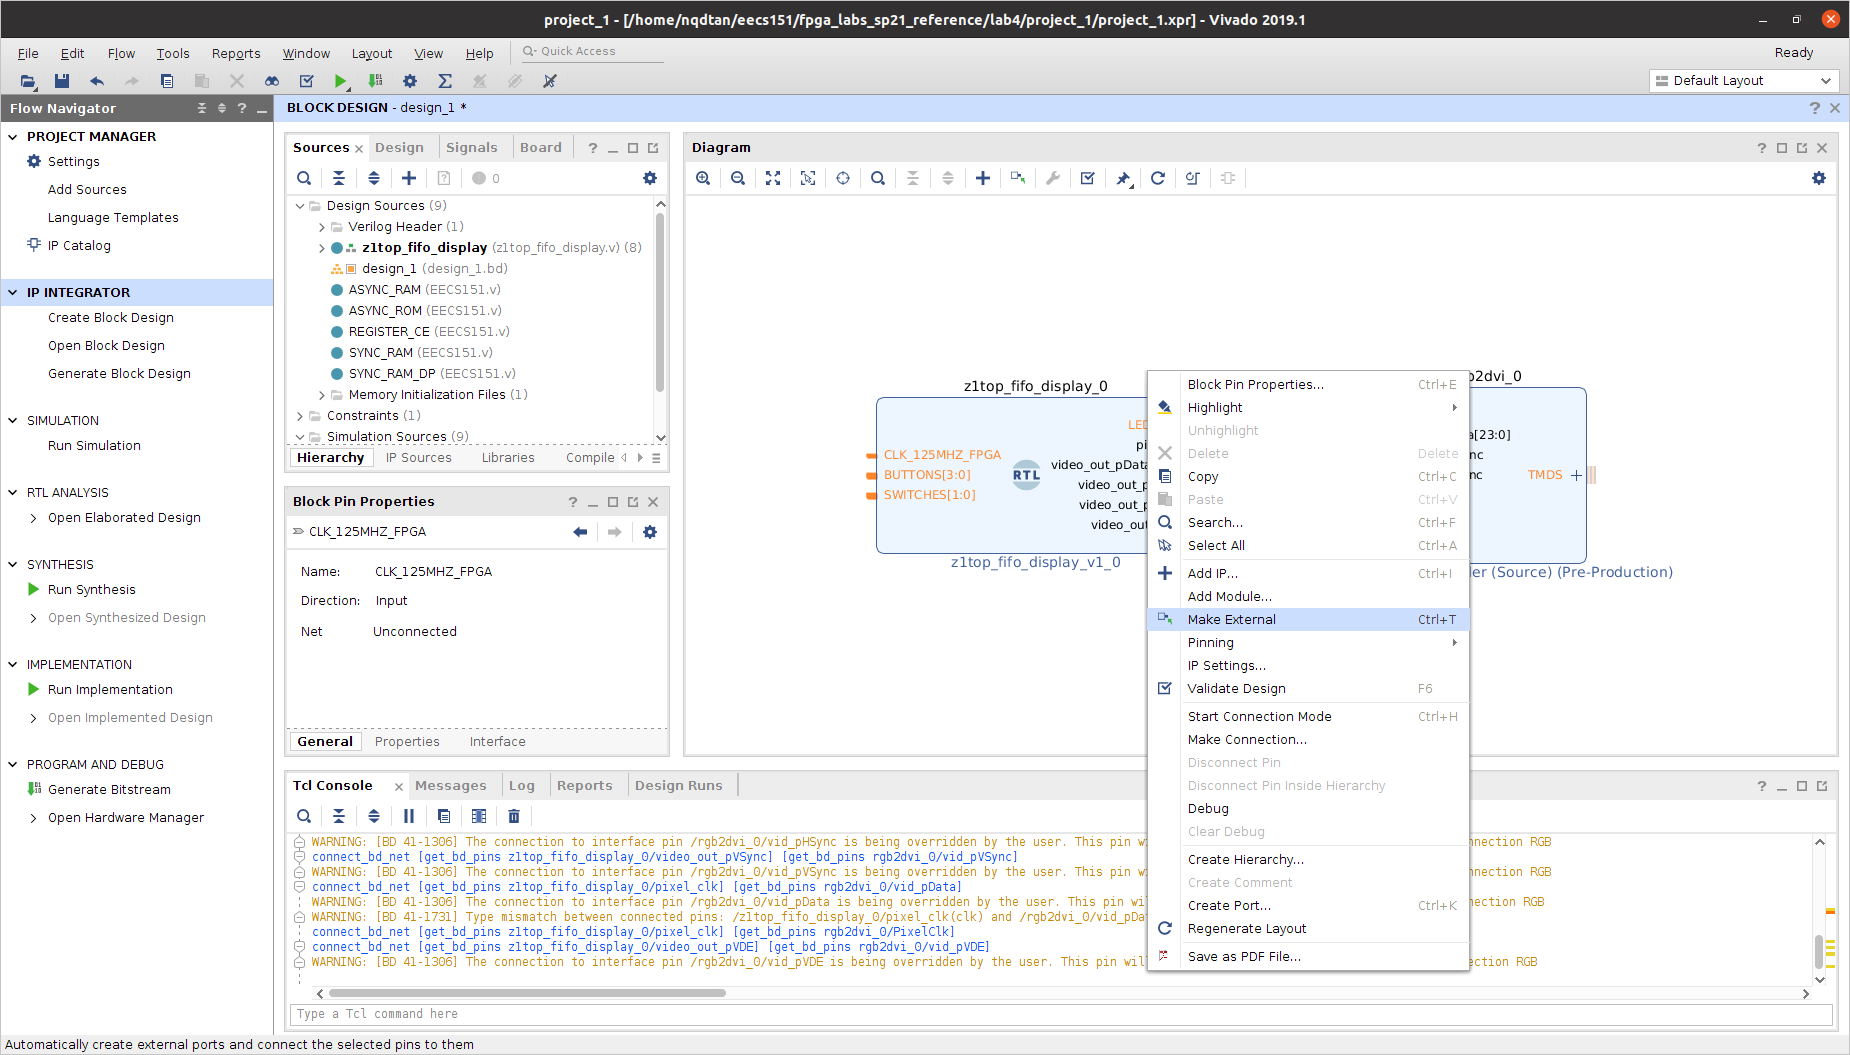
\includegraphics[width=0.7\textwidth]{figs/bd4.png}}
\end{center}

Rename the external IO ports as follows (click on an external port, then on the \texttt{External Port Properties} pane, modify its name in the \texttt{Name} box)

\texttt{CLK\_125MHZ\_FPGA\_0} to \texttt{CLK\_125MHZ\_FPGA}

\texttt{SWITCHES[1:0]\_0} to \texttt{SWITCHES[1:0]}

\texttt{BUTTONS[3:0]\_0} to \texttt{BUTTONS[3:0]}

\texttt{LEDS[5:0]\_0} to \texttt{LEDS[1:0]}

This ensures that they match the ports' names specified in the constraint file.

Basically, the idea is that the block design is the top-level module, and the IPs are the children modules instantiated internally.

The next step is to actually create an HDL wrapper for our block design, and set it as the top-level module so that we can synthesize and implement it as similar to how we did for the RTL modules in previous lab exercises. We can let Vivado manage wrapper and auto-update.

\begin{center}
\fbox{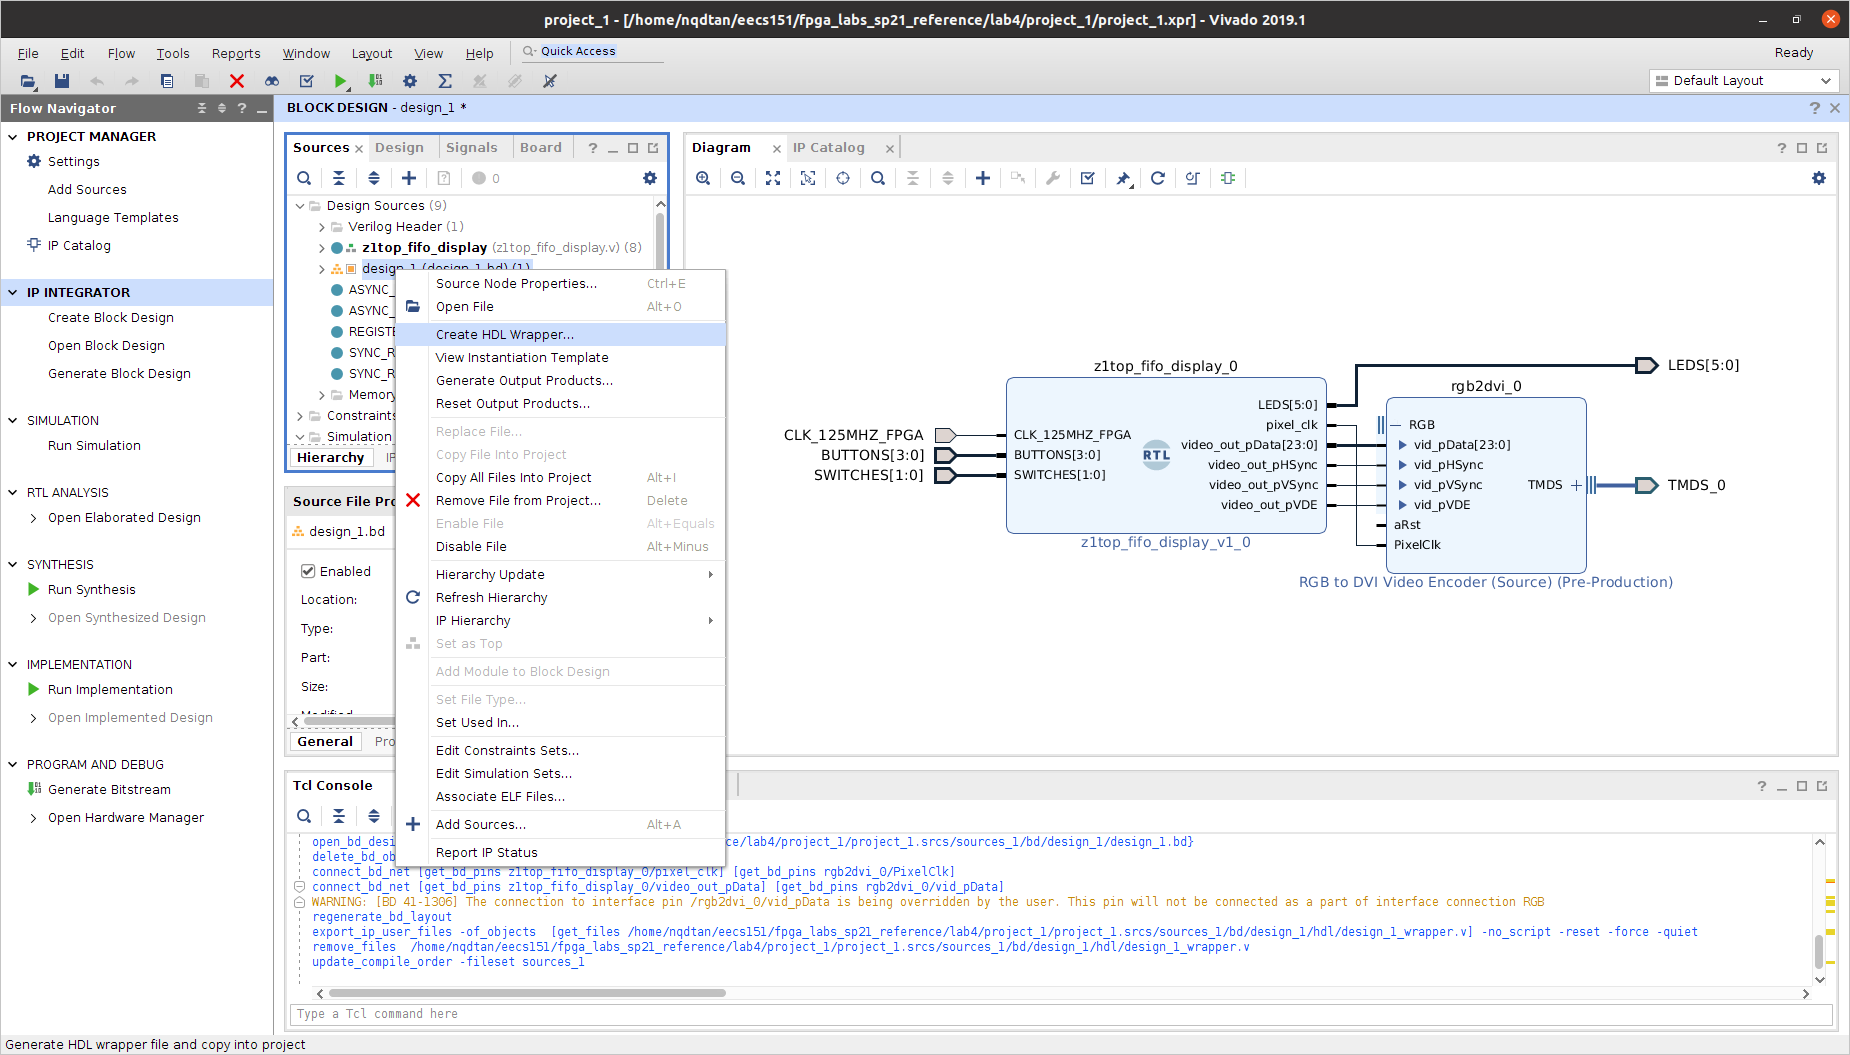
\includegraphics[width=0.7\textwidth]{figs/bd5.png}}
\end{center}

Click on the \texttt{rgb2dvi} IP, a window with the IP setting will pop up. For the \emph{TMDS Clock Range}, choose \emph{< 80MHz} since we use a 40MHz pixel clock in this design.

\begin{center}
\fbox{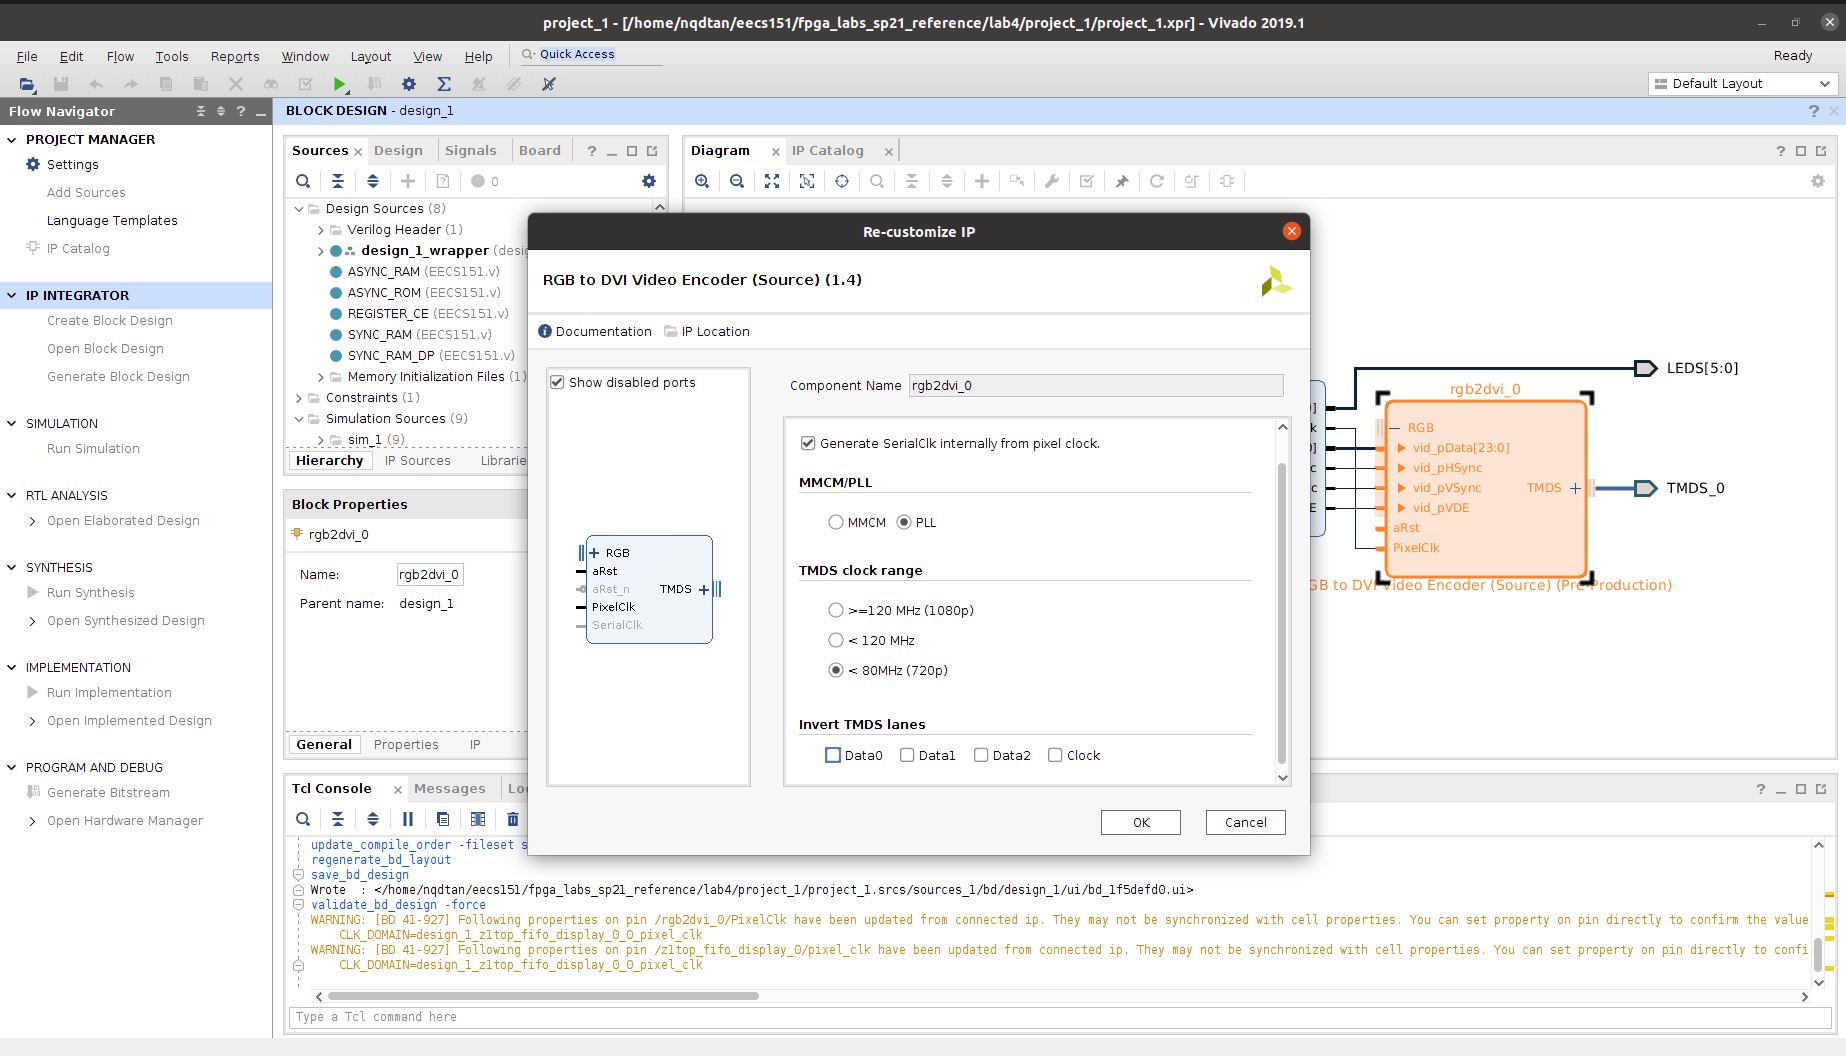
\includegraphics[width=0.7\textwidth]{figs/bd7.png}}
\end{center}

In the \texttt{Diagram} window, you can also click on the \texttt{Regenerate Layout} button to let the tool automatically shifting the IP blocks and their connection for better visualization. Click \texttt{Validate Design} button to check for any outstanding issues in your design. If not, you can proceed to generate bitstream as usual. Note that your top-level module is now \verb|design_1_wrapper|, instead of the \verb|z1top_fifo_display|.

\begin{center}
\fbox{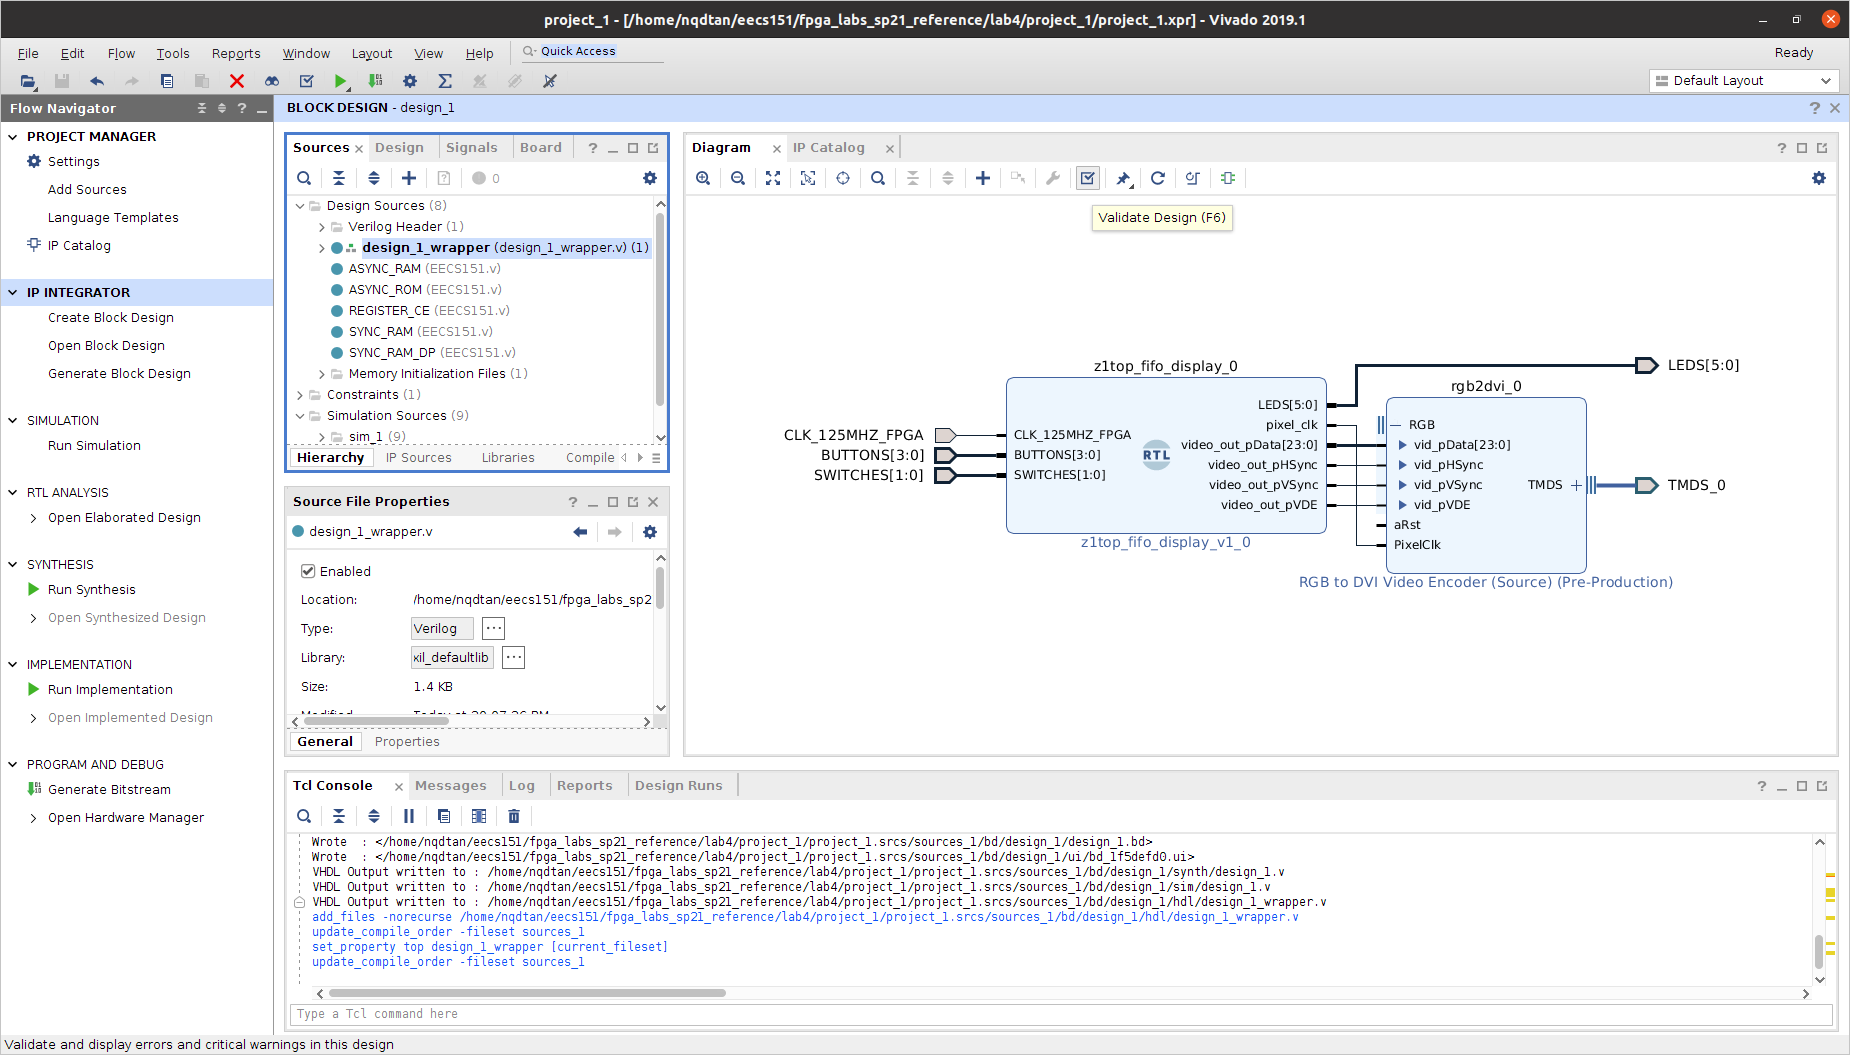
\includegraphics[width=0.7\textwidth]{figs/bd6.png}}
\end{center}

Remember that whenever you change an RTL source file, click \textbf{Refresh Changed Modules} so that the changes are effective before generating bitstream.

%\newpage
\section*{Acknowlegement}
This lab is the result of the work of many EECS151/251 GSIs over the years including:
\begin{itemize}
\item Sp12: James Parker, Daiwei Li, Shaoyi Cheng
\item Sp13: Shaoyi Cheng, Vincent Lee
\item Fa14: Simon Scott, Ian Juch
\item Fa15: James Martin
\item Fa16: Vighnesh Iyer
\item Fa17: George Alexandrov, Vighnesh Iyer, Nathan Narevsky
\item Sp18: Arya Reais-Parsi, Taehwan Kim
\item Fa18: Ali Moin, George Alexandrov, Andy Zhou
\item Sp19: Christopher Yarp, Arya Reais-Parsi
\item Fa19: Cem Yalcin, Rebekah Zhao, Ryan Kaveh, Vighnesh Iyer
\item Sp20: Tan Nguyen
\item Fa20: Charles Hong, Kareem Ahmad, Zhenghan Lin

\end{itemize}

\end{document}
